\section{Prehľad riešenia na vysokej úrovni}

Navrhnuté riešenie pozostáva z modulárneho systému na báze DT, ktorého cieľom je analyzovať a klasifikovať správanie 5G siete v kontrolovanom prostredí. Vytvorené DT simuluje vybrané komponenty reálnej siete a umožňuje generovanie syntetických dát, ich zber, spracovanie a následnú aplikáciu modelov strojového učenia. Architektúra systému bola navrhnutá s dôrazom na rozšíriteľnosť, modularitu a experimentálnu reprodukovateľnosť.

Open5GS je open-source implementácia 5G jadra siete, ktorá slúži ako základná riadiaca infraštruktúra pre prichádzajúce spojenia. V navrhnutom riešení zodpovedá za autentifikáciu zariadení, správu session a prideľovanie IP adries.

UERANSIM je emulátor RAN prístupu, ktorý generuje simulovaných používateľov (UE), ktorí sa pripájajú do siete (pozri Obr. \ref{fig:architecture}) cez definované scénare. Umožňuje flexibilne konfigurovať počet zariadení, typy prevádzky a časovanie spojení.

\begin{figure}[H]
    \centering
    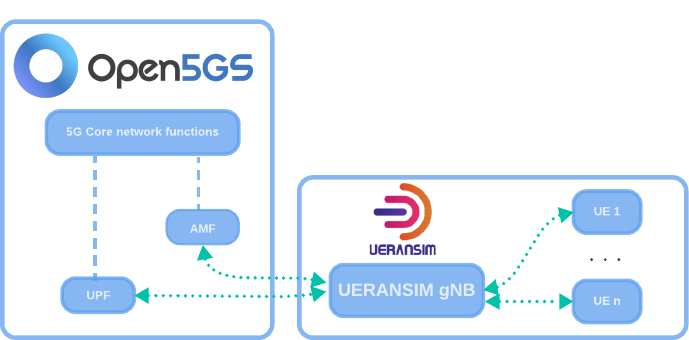
\includegraphics[width=0.75\linewidth]{assets//images/core-ue.png}
    \caption[Architektúra komponentov Open5GS a UERANSIM]{Architektúra jednotlivých komponentov Open5GS a UERANSIM a ich vzájomné prepojenie. Open5GS je rozdelené na riadiacu rovinu a rovinu užívateľských dát a obe tieto roviny sú napojené na gNB, ku ktorým sa môžu pripájať zariadenia.}
    \label{fig:architecture}
\end{figure}

Monitorovacia infraštruktúra pozostáva z nástrojov Prometheus, Grafana, Promtail a logwatcher.py. Prometheus zberá metriky zo siete a systémových zdrojov, ktoré sú vizualizované pomocou Grafany. Logwatcher je vlastný Python skript, ktorý analyzuje logy z Open5GS a exportuje vlastné metriky ako napr. počet aktívnych UE či SUCI identifikátory.

Skripty na simuláciu scenárov (UC) slúžia na spúšťanie preddefinovaných testovacích situácií. Každý UC definuje počet zariadení, objem prenesených dát a časovanie spojení, čím vytvára realistické syntetické zaťaženie siete.

Predspracovanie dát a výber metrík (EDA, preprocessing, feature selection) boli vykonané raz pred trénovaním modelu, s cieľom optimalizovať vstup pre model strojového učenia. Výber metrických premenných bol podporený metódami založenými na rozhodovacích stromoch a permutačnej dôležitosti.

Modely strojového učenia boli implementované pomocou LSTM modelov, ktoré sú vhodné pre sekvenčné dáta. Model bol natrénovaný na syntetických dátach a neskôr testovaný na dátach z reálnej siete.

\begin{figure}[H]
    \centering
    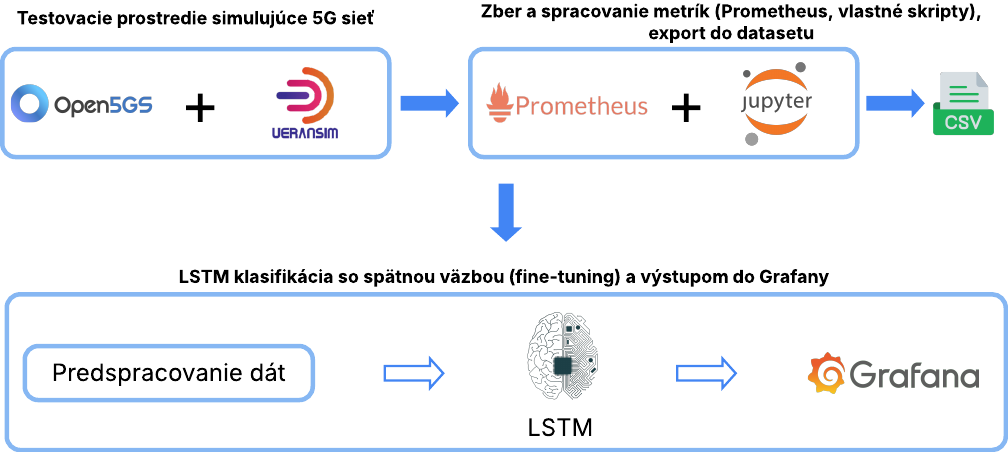
\includegraphics[width=0.95\linewidth]{assets//images/arch2.png}
    \caption{Zariadenia generované pomocou UERANSIM sa pripájajú k jadru siete v Open5GS, ktoré loguje udalosti a vystavuje metriky. Tieto údaje sú zbierané pomocou Promethea a logwatcher.py skriptu. Výstupy sú agregované do datasetu, ktorý sa ďalej spracúva v prostredí Jupyter Notebook. Po spracovaní sa dáta využívajú na trénovanie a testovanie modelov strojového učenia. Vizualizácia metrických údajov prebieha súbežne v Grafane.}
    \label{fig:arch}
\end{figure}

Modularita kontajnerizovaného riešenia založeného na Docker Compose umožňuje jednoduché nasadenie a replikáciu prostredia. Open-source komponenty boli zvolené kvôli dostupnosti a možnosti detailnej konfigurácie siete. Použitie syntetických scenárov poskytuje kontrolu nad testovaným správaním bez rizika ovplyvnenia reálnej prevádzky. LSTM siete boli zvolené vďaka schopnosti modelovať časové závislosti, ktoré sú kľúčové pri klasifikácii sieťového správania. Kombinácia reálneho a syntetického vstupu umožňuje overiť možnosti generalizácie modelov v telekomunikačnom prostredí.